\begin{applicationActivities}

\begin{definition}
A \term{linear transformation} (also known as a \term{linear map})
is a map between vector spaces that preserves the vector space operations.
More precisely, if \(V\) and $W$ are vector spaces, a map
\(T:V\rightarrow W\) is called a linear transformation if
\begin{enumerate}
\item \(T(\vec{v}+\vec{w}) = T(\vec{v})+T(\vec{w})\)
      for any \(\vec{v},\vec{w} \in V\).
\item \(T(c\vec{v}) = cT(\vec{v})\)
      for any \(c \in \IR,\vec{v} \in V\).
\end{enumerate}
In other words, a map is linear when vector space operations
can be applied before or after the transformation without affecting the result.
\end{definition}

\begin{definition}
Given a linear transformation \(T:V\to W\),
\(V\) is called the \term{domain} of \(T\) and
\(W\) is called the \term{co-domain} of \(T\).

\begin{center}
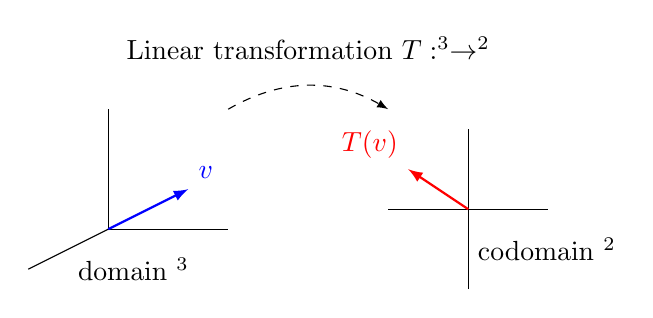
\begin{tikzpicture}[x=0.2in,y=0.2in]
  \begin{scope}[shift={(0,0)}]
    \draw (0,0) -- (3,0);
    \draw (0,0) -- (0,3);
    \draw (0,0) -- (-2,-1);
    \draw[thick,-latex,blue] (0,0) -- (2,1)
          node[anchor=south west] {\(\vect v\)};
    \node[anchor=west] at (-1,-1) {domain \(\IR^3\)};
  \end{scope}
  \draw[dashed,-latex] (3,3) to [bend left=30] (7,3);
  \node[anchor=south] at (5,4) {Linear transformation \(T:\IR^3\to\IR^2\)};
  \begin{scope}[shift={(9,0.5)}]
    \draw (-2,0) -- (2,0);
    \draw (0,-2) -- (0,2);
    \draw[thick,-latex,red] (0,0) -- (-1.5,1)
          node[anchor=south east] {\(T(\vect v)\)};
    \node[anchor=west] at (0,-1) {codomain \(\IR^2\)};
  \end{scope}
\end{tikzpicture}
\end{center}
\end{definition}

\begin{example}
Let \(T : \IR^3 \rightarrow \IR^2\) be given by
\[
  T\left(\begin{bmatrix} x \\ y \\ z \end{bmatrix} \right)
=
  \begin{bmatrix} x-z \\ 3y \end{bmatrix}
\]

To show that \(T\) is linear, we must verify...
\[
  T\left(
    \begin{bmatrix} x \\ y \\ z \end{bmatrix} +
    \begin{bmatrix} u \\ v \\ w \end{bmatrix}
  \right)
=
  T\left(
    \begin{bmatrix} x+u \\ y+v \\ z+w \end{bmatrix}
  \right) =
  \begin{bmatrix} (x+u)-(z+w) \\ 3(y+v) \end{bmatrix}
\]
\[
  T\left(
    \begin{bmatrix} x \\ y \\ z \end{bmatrix}
  \right) + T\left(
    \begin{bmatrix} u \\ v \\ w \end{bmatrix}
  \right)
=
  \begin{bmatrix} x-z \\ 3y \end{bmatrix} +
  \begin{bmatrix} u-w \\ 3v \end{bmatrix}=
  \begin{bmatrix} (x+u)-(z+w) \\ 3(y+v) \end{bmatrix}
\]
And also...
\[
  T\left(c\begin{bmatrix} x \\ y \\ z \end{bmatrix} \right)
=
  T\left(\begin{bmatrix} cx \\ cy \\ cz \end{bmatrix} \right)
=
  \begin{bmatrix} cx-cz \\ 3cy \end{bmatrix}
\text{ and }
  cT\left(\begin{bmatrix} x \\ y \\ z \end{bmatrix} \right)
=
  c\begin{bmatrix} x-z \\ 3y \end{bmatrix}
=
  \begin{bmatrix} cx-cz \\ 3cy \end{bmatrix}
\]

Therefore \(T\) is a linear transformation.
\end{example}

\begin{example}
Let \(T : \IR^2 \rightarrow \IR^4\) be given by
\[
  T\left(\begin{bmatrix} x \\ y \end{bmatrix} \right)
=
  \begin{bmatrix} x+y \\ x^2 \\ y+3 \\ y-2x \end{bmatrix}
\]

To show that \(T\) is not linear, we only need to find one
counterexample.
\[
  T\left(
    \begin{bmatrix} 0 \\ 1 \end{bmatrix} +
    \begin{bmatrix} 2 \\ 3 \end{bmatrix}
  \right)
=
  T\left(
    \begin{bmatrix} 2 \\ 4 \end{bmatrix}
  \right) =
  \begin{bmatrix} 6 \\ 4 \\ 7 \\ 0 \end{bmatrix}
\]
\[
  T\left(
    \begin{bmatrix} 0 \\ 1 \end{bmatrix}
  \right) + T\left(
    \begin{bmatrix} 2 \\ 3\end{bmatrix}
  \right)
=
  \begin{bmatrix} 1 \\ 0 \\ 4 \\ 1 \end{bmatrix} +
  \begin{bmatrix} 5 \\ 4 \\ 6 \\ -1 \end{bmatrix} =
  \begin{bmatrix} 6 \\ 4 \\ 10 \\ 0 \end{bmatrix}
\]

Since the resulting vectors are different,
\(T\) is a linear transformation.
\end{example}

\begin{activity}{5}
Show that \(T : \IR^2 \rightarrow \IR^4\) defined by
\[
  T\left(\begin{bmatrix} x \\ y \end{bmatrix} \right)
=
  \begin{bmatrix} x+y \\ x^2 \\ y+3 \\ y-2x \end{bmatrix}
\]
is not linear by showing that
\(
  2T\left(\begin{bmatrix} 1 \\ 1 \end{bmatrix} \right)
\not=
  T\left(2\begin{bmatrix} 1 \\ 1 \end{bmatrix} \right)
\).
\end{activity}

\begin{fact}
A map between Euclidean spaces \(T:\IR^n\to\IR^m\) is linear
exactly when every component of the output is a linear combination
of the variables of \(\IR^n\).
\end{fact}

\begin{example}
You can quickly identify
\[
  T\left(\begin{bmatrix} x \\ y \\ z \end{bmatrix} \right)
=
  \begin{bmatrix} x-z \\ 3y \end{bmatrix}
\]
as linear because \(x-z\) and \(3y\) are linear combinations
of \(x,y,z\).

But
\[
  T\left(\begin{bmatrix} x \\ y \end{bmatrix} \right)
=
  \begin{bmatrix} x+y \\ x^2 \\ y+3 \\ y-2x \end{bmatrix}
\]
cannot be linear because \(x^2\) and \(y+3\) are not linear
combinations of \(x,y\) (even though \(x+y\) and \(y-2x\) are).
\end{example}

\begin{activity}{3}
  Recall the following rules from calculus, where \(D:\P\to\P\)
  is the derivative map defined by \(D(f)=\frac{df}{dx}\) for each
  polynomial \(f\).
  \[
    D(f+g)=\frac{df}{dx}+\frac{dg}{dx}
  \]
  \[
    D(cf)=c\frac{df}{dx}
  \]
  What can we conclude from these rules?
  \begin{enumerate}[a)]
    \item \(\P\) is not a vector space
    \item \(D\) is a linear map
    \item \(D\) is not a linear map
  \end{enumerate}
\end{activity}


\begin{activity}{12}
Consider the following two polynomial maps.

\[S: \P^4 \rightarrow \P^3 \text{ given by } S(f(x)) = 2f'(x)-f''(x)\]
\[T: \P^2 \rightarrow \P^2 \text{ given by } T(f(x)) = f'(x)+x^2\]

\begin{subactivity}
  Compare \(S(x^2+x)\) with \(S(x^2)+S(x)\), and
  compare \(T(x^2+x)\) with \(T(x^2)+T(x)\). Which of these maps
  is definitely not linear?
\end{subactivity}
\begin{subactivity}
  Verify that \(S(f+g)=2f'(x)+2g'(x)-f''(x)-g''(x)\) is equal
  to \(S(f)+S(g)\) for all polynomials \(f,g\).
\end{subactivity}
\begin{subactivity}
  Verify that \(S(cf)=cS(f)\) for all real numbers \(c\) and polynomials \(f\).
  Is \(S\) linear?
\end{subactivity}
\end{activity}

\end{applicationActivities}
